\clearpage
\begin{flushright}
	\textit{Лекция №11}
	\textit{2015.10.20}
\end{flushright}

\chapter{Взаимодействие параллельных процессов}

Чтобы не терять значение разделяемой переменной, необходимо обеспечить монопольный доступ (когда процесс получает доступ к критической секции (КС) по разделяемой переменной, то системой больше ни какой процесс не сможет получить доступ к этой же КС.) 

Монопольльный доступ обеспечивается методами взаимоисключения, делятся на:
\begin{enumerate}
    \item программные
    \item аппаратные
    \item с помощью семафоров
    \item мониторы.
\end{enumerate} 

В общем случае задача взаимоисключения решается для N процессов.

\section{Программная реализация}

С использованием флага, который проверяется в цикле.

\begin{figure}[H]
    \centering
    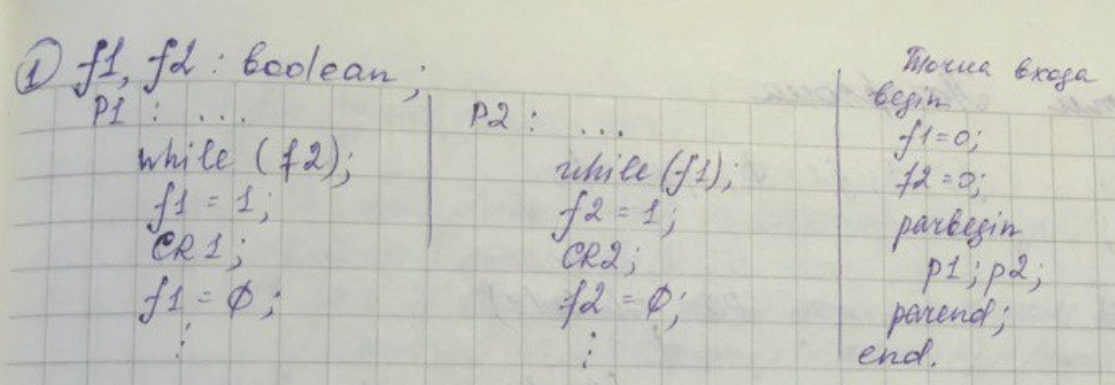
\includegraphics[width=\textwidth]{listing/1.png}
    \caption{вариант 1}
    \label{listing:prog_flag}
\end{figure}

В \ref{listing:prog_flag} второй процесс мог не успеть установить флаг, тогда первый процесс также пройдет цикл while, следовательно сново получаем одновременный доступ.

\begin{figure}[H]
    \centering
    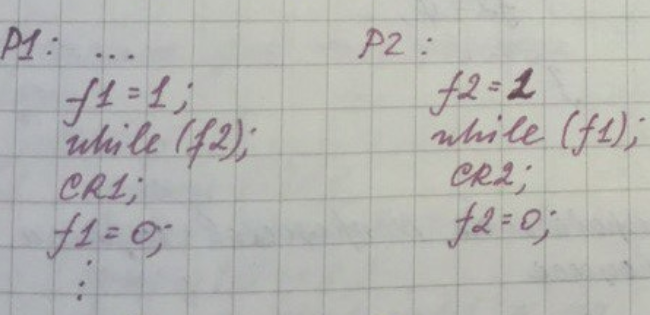
\includegraphics[width=\textwidth]{listing/2.png}
    \caption{вариант 2}
    \label{listing:prog_flag_2}
\end{figure}

В \ref{listing:prog_flag_2} зацикливание в проверке флага!

\subsection{Алгоритм Дейкера}

Дейкер ввел дополнительную переменную ("чья очередь?") и 2 флага. Алгоритм обеспечивает взаимоисключения.

\begin{figure}[H]
    \centering
    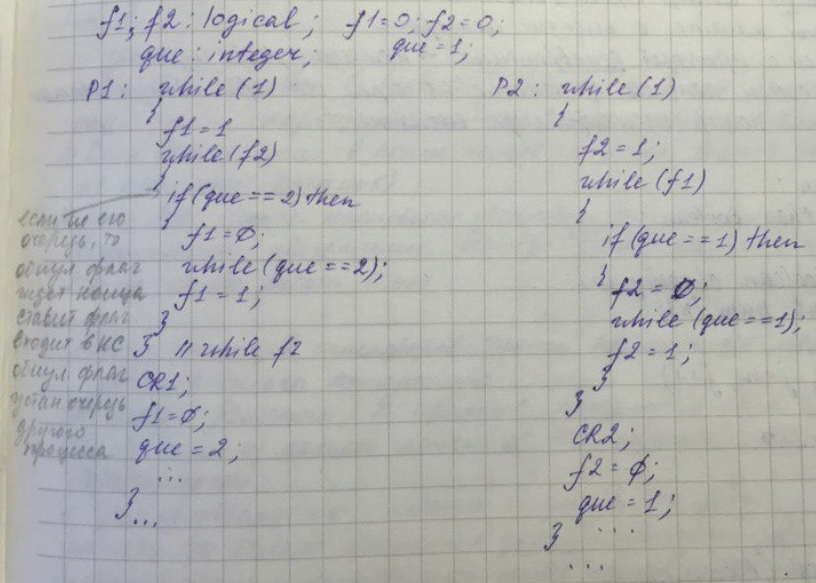
\includegraphics[width=\textwidth]{listing/3.png}
    \caption{Алгоритм Дейкера}
\end{figure}

\subsection{Алгоритм Петерсона}

Этот алгоритм можно пролонгировать на N процессов и рассматривать значение "que" - как номер процесса.

\begin{figure}[H]
    \centering
    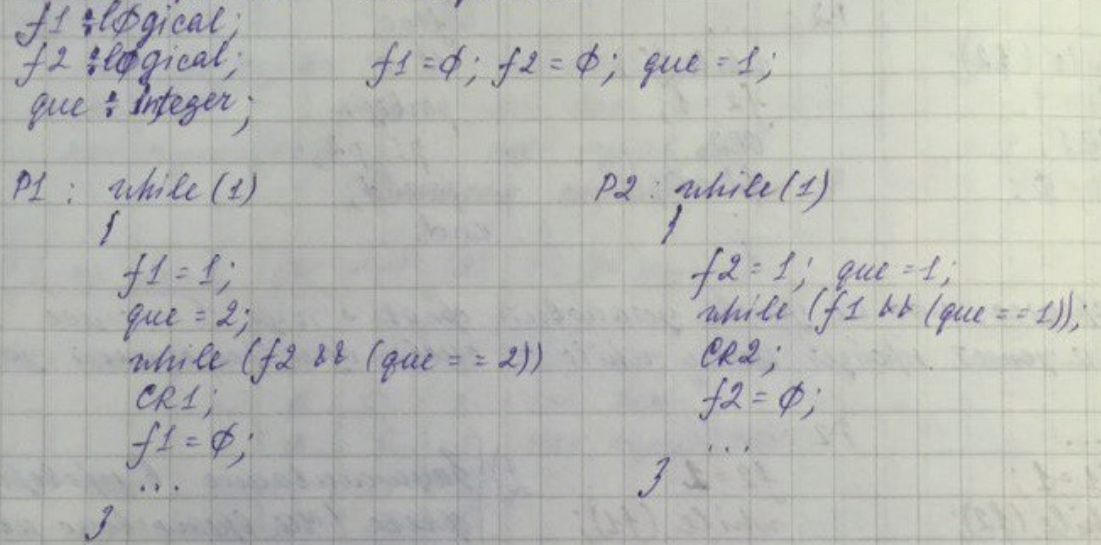
\includegraphics[width=\textwidth]{listing/4.png}
    \caption{Алгоритм Петерсона}
\end{figure}

\subsection{Алгоритм Bakery (Лампорта)}

Решает задачу взаимоисключения для N процессов. Каждому приходящему клиенту выдается жетон с номером. Каждому новому - номер строго больше. Продавец обслуживает клиента с меньшим номером. Если 2 клиента приходят одновременно, то возникает коллизия, которую нужно разрешить: процессы получают одинаковые номера, но при обслуживании, процесс, у которого номер идентификатора меньше

?????????????????????????????????????????????????????????????\\
?????????????????????????????????????????????????????????????\\
?????????????????????????????????????????????????????????????\\


